\documentclass{article}

    \usepackage{fancyhdr}
    \usepackage{extramarks}
    \usepackage{amsmath}
    \usepackage{amsthm}
    \usepackage{amsfonts}
    \usepackage{tikz}
    \usepackage{amssymb}
    \usepackage{subcaption}
    \usepackage{blkarray}
    \usetikzlibrary{arrows, automata}
    \usepackage{forest}
    \usetikzlibrary{chains,positioning} %

    \usepackage{algorithm}
    \usepackage{algorithmicx}

    \usepackage{mathtools}
    \usepackage{bm}
    \usepackage{esvect}
    \usepackage{graphicx}



    

    \makeatletter
    \def\BState{\State\hskip-\ALG@thistlm}
    \makeatother


    \newcommand{\Mod}[1]{\ (\mathrm{mod}\ #1)}

    






    \usepackage{tabulary}

\usepackage[newcommands]{ragged2e}

    \usetikzlibrary{trees}

    \newcommand{\question}{\textbf{Question:}}
    \newcommand{\answer}{\textbf{Answer:}}
    \newcommand{\modx}{\;(\bmod\;}

    


    \usetikzlibrary{decorations.markings}
    \tikzstyle{vertex}=[circle, draw, inner sep=0pt, minimum size=6pt]
    \newcommand{\vertex}{\node[vertex]}

    
    \usepackage{amsmath}
    \usepackage{algorithm}
    \usepackage[noend]{algpseudocode}
    \usepackage[utf8]{inputenc}
    \usepackage{enumerate}
    \usepackage{geometry}
    \usepackage{mathtools}
    \usepackage{parskip}
    \usepackage{xifthen, xparse}
    
    \algdef{SE}[SUBALG]{Indent}{EndIndent}{}{\algorithmicend\ }%
    \algtext*{Indent}
    \algtext*{EndIndent}
    
    
    
    \usetikzlibrary{automata,positioning}
    
    %
    % Basic Document Settings
    %
    
    \topmargin=-0.45in
    \evensidemargin=0in
    \oddsidemargin=0in
    \textwidth=6.5in
    \textheight=9.0in
    \headsep=0.25in
    
    \linespread{1.1}
    
    \pagestyle{fancy}
    \lhead{\hmwkAuthorName}
    \chead{\hmwkClass\ \hmwkTitle}
    \rhead{\firstxmark}
    \lfoot{\lastxmark}
    \cfoot{\thepage}
    
    \renewcommand\headrulewidth{0.4pt}
    \renewcommand\footrulewidth{0.4pt}
    
    \setlength\parindent{0pt}
    
    %
    % Create Problem Sections
    %
    
    \newcommand{\enterProblemHeader}[1]{
        \nobreak\extramarks{}{Problem \arabic{#1} continued on next page\ldots}\nobreak{}
        \nobreak\extramarks{Problem \arabic{#1} (continued)}{Problem \arabic{#1} continued on next page\ldots}\nobreak{}
    }
    
    \newcommand{\exitProblemHeader}[1]{
        \nobreak\extramarks{Problem \arabic{#1} (continued)}{Problem \arabic{#1} continued on next page\ldots}\nobreak{}
        \stepcounter{#1}
        \nobreak\extramarks{Problem \arabic{#1}}{}\nobreak{}
    }
    
    \newcommand\rowop[1]{\scriptstyle\smash{\xrightarrow[\vphantom{#1}]{\mkern-4mu#1\mkern-4mu}}}
    
    \DeclareDocumentCommand\converttorows%
    {>{\SplitList{,}}m}%
    {\ProcessList{#1}{\converttorow}}
    \NewDocumentCommand{\converttorow}{m}
    {\ifthenelse{\isempty{#1}}{}{\rowop{#1}}\\}
    
    \DeclareDocumentCommand \rowops{m}
    {\;
     \begin{matrix}
    \converttorows {#1}
     \end{matrix}
     \; }
    
    \setcounter{secnumdepth}{0}
    \newcounter{partCounter}
    \newcounter{homeworkProblemCounter}
    \setcounter{homeworkProblemCounter}{1}
    \nobreak\extramarks{Problem \arabic{homeworkProblemCounter}}{}\nobreak{}
    
    %
    % Homework Problem Environment
    %
    % This environment takes an optional argument. When given, it will adjust the
    % problem counter. This is useful for when the problems given for your
    % assignment aren't sequential. See the last 3 problems of this template for an
    % example.
    %
    \newenvironment{homeworkProblem}[1][-1]{
        \ifnum#1>0
            \setcounter{homeworkProblemCounter}{#1}
        \fi
        \section{Problem \arabic{homeworkProblemCounter}}
        \setcounter{partCounter}{1}
        \enterProblemHeader{homeworkProblemCounter}
    }{
        \exitProblemHeader{homeworkProblemCounter}
    }
    
    %
    % Homework Details
    %   - Title
    %   - Due date
    %   - Class
    %   - Section/Time
    %   - Instructor
    %   - Author
    %
    
    \newcommand{\hmwkTitle}{SOFTENG211 Assignment \#3}
    \newcommand{\hmwkClass}{S.E. Theory}
    \newcommand{\hmwkAuthorName}{\textbf{Nisarag Bhatt}}

    
    %
    % Title Page
    %
    
    \title{
        \vspace{2in}
        \textmd{\textbf{\hmwkClass:\ \hmwkTitle}}\\
        \vspace{3in}
    }
    
    \author{\hmwkAuthorName}
    \date{}
    
    \newtheorem{theorem}{Theorem}

    \renewcommand{\part}[1]{\textbf{\large Part \Alph{partCounter}}\stepcounter{partCounter}\\}
    
    %
    % Various Helper Commands
    %
    
    % Useful for algorithms
    \newcommand{\alg}[1]{\textsc{\bfseries \footnotesize #1}}
    
    % For derivatives
    \newcommand{\deriv}[1]{\frac{\mathrm{d}}{\mathrm{d}x} (#1)}
    
    % For partial derivatives
    \newcommand{\pderiv}[2]{\frac{\partial}{\partial #1} (#2)}
    
    % Integral dx
    \newcommand{\dx}{\mathrm{d}x}
    
    % Alias for the Solution section header
    \newcommand{\solution}{\textbf{\large Solution}}
    
    % Probability commands: Expectation, Variance, Covariance, Bias
    \newcommand{\E}{\mathrm{E}}
    \newcommand{\Var}{\mathrm{Var}}
    \newcommand{\Cov}{\mathrm{Cov}}
    \newcommand{\Bias}{\mathrm{Bias}}
    
    \begin{document}

    \maketitle
    
    \pagebreak

    \begin{homeworkProblem}
        
        \question  

        Let $A$ be a set with exactly $n$ elements.  
        
        Consider the following two sets: $X = \{f ~|~ f: A \to \{0, 1\} \} $ and $Y=\{u~|~u ~ \text{is a binary string of length} ~n \}$.

        Show that there is a bijection from $X$ onto $Y$.

        \answer

        Since $X,Y$ are both finite sets then the existence of a bijection means they have the same number of elements.

        We seek to prove $|X|=|Y|$ for there to exist a bijection from $X$ onto $Y$. 

        \begin{proof}
            
            First we consider the cardinality of $|X|$. By definition $A$ has $n$ elements and for every element in $A$ you can choose $2$ options either $0,1$ so we conclude there are $\underbrace{2 \cdot 2 \cdot ... \cdot 2}_{n ~ \text{times}} = 2^n$ functions
            in the set $X$ that map $A \to \{0, 1\}$  hence $|X| = 2^n$.

            Now we consider the cardinality of $|Y|$. $Y$ is simply all the possible binary strings of length $n$. 
            
            One may notice that for $n=0$ we have that there is $2^0=1$ binary string (the empty string), for $n=1$ we have that there is $2^1=2$ binary strings ($0, 1$) and so forth.

            Consider the statement $P(n) = \text{"There are $2^n$ binary strings of length $n$"}$. We continue to prove $P(n)$ by induction. 

            \textbf{Base Case}: $n=0$: If $n=0$ then $P(0) =$ empty string. $\checkmark$

            \textbf{Inductive Hypothesis}: Suppose for an arbitrary $n$, assume $P(n)$ is true.
            
            \textbf{Inductive Step}: Want to show $P(n) \implies P(n+1)$:  Consider the set of all binary strings of length $n+1$ (Call this set $\phi$). Note that all binary strings either end in $1$ or $0$. 

            Split $\phi$ up into two sets $\alpha,\beta$: 

            \begin{itemize}
                \item $\alpha$ consists of all binary strings of length $n+1$ that end with $0$ 
                \item $\beta$ consists of all binary strings of length $n+1$ that end with $1$ 
            \end{itemize}

            One may also notice that $\alpha$ consists of arbitrary binary strings with length $n$ that end with $0$ so by Inductive Hypothesis there are $2^n$ of these strings.
            
            Similarly $\beta$ consists of arbitrary binary strings with length $n$ that end with $1$ so by Inductive Hypothesis there are $2^n$ of these strings.

            We can now see that $|\phi| = |\alpha| + |\beta| = 2^n + 2^n = 2^n(1+1)=2^{n+1}$. So there are exactly $2^{n+1}$ binary strings of length $n+1$ so $P(n+1)$ holds.

            So $P(n) \implies P(n+1)$, Hence $P(n)$ is true for all $n \in \mathbb{N}$.

            From the proof by induction we now know that $|Y| = 2^n$.

            Since $|X|=|Y|$, this must mean there is a bijection from $X$ onto $Y$. (See proof of this in Question 2 Part 1 (if $n=m$ then there is a bijection from $A$ onto $B$))
        \end{proof}


    \end{homeworkProblem}
    
    \pagebreak

    \begin{homeworkProblem}
        
        \question  

        Let $A$ and $B$ be two finite sets with exactly $n$ and $m$ elements, respectively.  
        
        Show the following:

        \answer

        \begin{enumerate}
            \item There is a bijection from $A$ onto $B$ if and only if $n=m$
                \begin{itemize}
                    \item $\Rightarrow$ 
                    \begin{proof}
                        If there is a bijection from $A$ onto $B$ then there exists a bijective function $f: A \to B$

                        For the sake of contradiction assume that $n \neq m$.

                        Case $1$: $n>m$ - Let $A=\{a_1,...,a_n\}$ and $B=\{b_1,...,b_m\}$. If $n>m$ then there exists elements $a_i, a_j \in A$ such that $a_i, a_j$ are mapped to an element $b_i \in B$. This means $f$ is not injective (since $f(x) = f(y)$ does not imply $x=y$) and hence not bijective. Contradiction. 

                        Case $2$: $n<m$ - Let $A=\{a_1,...,a_n\}$ and $B=\{b_1,...,b_m\}$. If $n<m$, then there exists an element in $b_i \in B$ such that $f(a_i) \neq b_i$. However this contradicts the fact that $f$ is surjective which further contradicts the fact that $f$ is bijective. 

                        Since in both cases we get a contradiction, we have that if there is a bijection from $A$ onto $B$ then $n=m$.
                    \end{proof}
                    \item $\Leftarrow$ \begin{proof}
                        If $n=m$ then consider the sets $A=\{a_1,...,a_n\}$ and $B=\{b_1,...,b_n\}$.

                        Suppose the exists a functions $f: A \to B$ such that $f$ maps $a_1 \to b_1$, $a_2 \to b_2$ and so forth until $a_n \to b_n$. 

                        This function is injective if $f(x)=f(y) \Rightarrow x=y$. For this function, if $f(a_i)=f(a_j)$, then it neccessary that $i=j$, since if $i \neq j$, $b_i \neq b_j$ by definition (of the way we defined the function). Therefore $f$ is bijective.
                        
                        This function is surjective if for every $y$ in the codomain, there exists an $x$ such that $f(x)=y$. In this case given a $b_i$, we have that there exists an $a_i$ such that $f(a_i)=b_i$ for every $i$ (where $0<i \leq n$). Therefore $f$ is surjective. 
                        
                        Since $f$ is injective and surjective then by definition $f$ must be bijective. Therefore if $n=m$, there exists a bijection from $A$ onto $B$. 

                    \end{proof}
                \end{itemize}
            \item Show that there is an injection from $A$ into $B$ if and only if $n \leq m$.
                \begin{itemize}
                    \item $\Rightarrow$ 
                    \begin{proof}
                        Suppose there exists an injective function $f: A \to B$ where $\forall a_i,a_j \in A, f(a_i)=f(a_j) \Rightarrow a_i = a_j.$

                        For the sake of contradiction assume $n>m$. 

                        Let $A=\{a_1,...,a_n\}$ and $B=\{b_1,...,b_m\}$. If $n>m$ then there exists elements $a_i, a_j \in A$ such that $a_i, a_j$ are mapped to an element $b_i \in B$. This means $f$ is not injective (since $f(x) = f(y)$ does not imply $x=y$). Contradiction. 

                        This must mean that that if there is an injection from $A$ into $B$ then $n \leq m$.
                    \end{proof}
                    \item $\Leftarrow$ \begin{proof}
                        We will prove that if $n \leq m$ then there is an injection from $A$ into $B$. 
                        
                        When $n=m$ trivially we have a bijection (see the proof for $\Leftarrow$ for Part $1$ of this question) and hence an injection from $A$ into $B$.
                        
                        So consider the case when $n<m$. 

                        Let $A=\{a_1, ..., a_n \}$ and $B=\{b_1,...,b_n,...,b_m\}$ 

                        Pick a subset of $B$ which contains $n$ elements ($B' = \{b_1, ... , b_n\}$). 
                        
                        Since $A$ and $B'$ both have $n$ elements, consider an explicit bijection $f:A \to B'$.

                        $f$ essentially maps $a_1 \to b_1$ , $a_2 \to b_2$, until $a_n \to b_n$. 
                        
                        (see the proof for $\Leftarrow$ for Part $1$ of this question to see that $f$ is a bijection). Since $f$ is a bijection it must also be injection. 

                        Now consider a function $g: B' \to B$ that sends every element to itself, note that $B'$ has $n$ elements and $B$ has $m$ elements. 

                        $g$ is injective because $B$ has $m$ elements and $B'$ has $n$ elements, since $n<m$ an injection exists since all elements in $B'$ are mapped to themselves in $B$
                        
                        So for all $f(b_i)=f(b_j)$ we will have $b_i=b_j$ since each element maps to itself. Any left over are left unmapped so injectivity still exists since no element in $B'$ maps to more than one element in $B$. 

                        Since $f: A \to B'$ and $g: B' \to B$. We consider the composition $g \circ f: A \to B$. We are required to prove $g \circ f$ is an injection to complete this proof. 
                        
                        \begin{proof}
                            Since $f(a)=f(b) \implies a=b$ and $g(a)=g(b) \implies a=b$

                            So $g(f(a)) = g(f(b)) \implies f(a)=f(b) \implies a=b$
                        \end{proof}

                        Since $g \circ f: A \to B$ is an injection, there must exist an injection from $A$ into $B$ if $n \leq m$.

                    \end{proof}
                \end{itemize}
        \end{enumerate}


    
        


    \end{homeworkProblem}
    
    \pagebreak

    \begin{homeworkProblem}
        
        \question  

        Let $A$ be a set with exactly $n$ elements. 
        
        Prove by induction that the number of bijective functions from $A$ into $A$ equals $n!$.

        Clearly state your  base  case,  inductive  hypothesis,  and  present  a  clear  inductive step.

        \answer

        \begin{proof}

            \centerline{$\forall n \in \mathbb{N} ~ P(n) = \text{"The number of bijective functions from $A$ into $A$ equals $n!$ where $A$ is a set with $n$ elements"}$}
        
            \textbf{Base Case}: $n=1$: If $n=1$ then $A$ has one element, trivially there only exists one function which maps that element to itself. $\checkmark$

            \textbf{Inductive Hypothesis}: Suppose for an arbitrary $n$, assume $P(n)$ is true. This means there for a set with $n$ elements we have that there exists $n!$ bijective functions to itself.

            \textbf{Inductive Step}: Consider a set with $n+1$ elements: $D = \{d_1, d_2, ..., d_n, d_{n+1}\}$

            Consider all the injective functions on this set. Split these functions into $n+1$ sets $K_{i}$ where the functions in $K_{i}$ are the injective functions that send $d_1$ to $d_i$.
            
            Note that the functions in $K_1$ send $d_1$ to $d_1$, so are determined by what the function does on the set of $n$ elements $\{d_2,...,d_{n+1}\}$. By our inductive hypothesis we have that 
            there exist $n!$ functions that do this. By this logic, each set $K_i$ has $n!$ elements. Since there $n+1$ sets of these $n!$ elements. 

            We then have that $\underbrace{n! + n! + ... + n!}_{n+1 ~\text{times}}= (n+1)n! = (n+1)!$. This means there exists $(n+1)!$ different functions that map $D$ into $D$. 

            Since we have proved $P(1)$ and $\forall n \in \mathbb{N}: P(n) \implies P(n+1)$. 
                
            We can thus conclude $\forall n \in \mathbb{N} : P(n)$ holds. 
            
        \end{proof}
    
        
           
    \end{homeworkProblem}
    
    \pagebreak

    \begin{homeworkProblem}
        
        \question  

        Prove, using the induction principle, that $3^{2n}-1$ is always divisible by  $8$  for  all  integers $n \geq 0$.   

        Clearly state your base case, inductive hypothesis, and present a clear inductive step.

        \answer

        \begin{proof}
            Consider $"P(n) = 8|3^{2n}-1"$, we seek to claim $P(n)$ holds for all integers $n \geq 0$

            \textbf{Base Case}: $n=0$: If $n=0$ then $P(0) = 8|3^{2 \cdot 0} - 1 =8|0$. Trivially $8|0$ hence $P(0)$ holds.

            \textbf{Inductive Hypothesis}: Suppose for an arbitrary $n$, assume $P(n)=8|3^{2n}-1$ is true.
            
            \textbf{Inductive Step}: 
            By the Inductive Hypothesis we have that $8|3^{2n}-1$ which means $3^{2n} - 1 = 8 \cdot m$ for some $m \in \mathbb{Z}$. So $3^{2n} = 8 \cdot m + 1$

            We now  consider the expression 
            \begin{align*}
                & 3^{2(n+1)}-1 \\ 
                &= 3^{2n+2}-1 \\ 
                &= 3^{2n}3^{2} -1  \\ 
                &= 3^{2n}(9) -1 \\
                &= (8 \cdot m + 1) \cdot 9  - 1  ~~~ \text{By IH} \\ 
                &= 72m + 9 - 1 \\
                &= 72m + 8 \\ 
                &= 8(9m + 1) \\ 
            \end{align*}
            
            Note that $9m+1$ is simply an integer hence $8 | 3^{2(n+1)}-1$ so $P(n+1)$ is true. 

            Since we have proved $P(0)$ and $\forall~\text{integers}~ n \geq 0: P(n) \implies P(n+1)$ 
            
            We can thus conclude $\forall~\text{integers}~ n \geq 0: P(n)$ holds. 
        \end{proof}

    
    \end{homeworkProblem}
    
    \pagebreak

    \begin{homeworkProblem}
        
        \question  

        On the set $\mathbb{Z}$ of integers consider the following relation $E$. 
        
        Pair $(x, y)$ is in $E$ if and only if either $(|x| \leq 10$ and $|y| \leq 10$ and $x \cdot y > 0)$ or $(x=y= 0)$ or $(|x|>10$ and $|y|>10)$.  
        
        Do the following:

        \begin{enumerate}
            \item Prove that $E$ is an equivalence relation.
            \item Describe all equivalence classes of $E$.
        \end{enumerate}

        \answer

        For $E$ to be an equivalence relation it must satisfy $3$ key properties:

        \begin{itemize}
            \item \textbf{Reflexive} \\
                Required to prove: For all $x \in \mathbb{Z}$, $xEx$ 
                \begin{proof}
                    Consider $x \in \mathbb{Z}$
                    \begin{itemize}
                        \item If $x=0$ then $x=x=0$ and hence $(x,x) \in E$.
                        \item If $|x| \leq 10$ and $x \neq 0$ then note that $x \cdot x \neq 0$ which means $(x,x) \in E$. 
                        \item If $|x| > 10$ then it must be the case $(x,x) \in E$. 
                    \end{itemize}
                \end{proof}
            \item \textbf{Symmetric} \\
                Required to prove: For all $x,y \in \mathbb{Z}$, if $xEy$ then $yEx$.
                \begin{proof}
                    Suppose that $xEy$ then it means $(x,y) \in E$; consider these cases: 
                    \begin{itemize}
                        \item If $x,y=0$ 
                            \begin{itemize}
                                \item If $x=y=0$ then it follows that $y=x=0$ therefore $yEx$
                            \end{itemize}
                        \item $x,y \neq 0$ 
                            \begin{itemize}
                                \item If $|x| ~ \text{and} ~ |y| > 10$ then it obviously follows $|y|, |x|>10$ and hence $yEx$.
                                \item If $|x| \leq 10 ~ \text{and} ~ |y| \leq 10$ 
                                    \begin{itemize}
                                        \item If $0 < x,y \leq 10$ (both positive) then $(x,y) \in E$. Since $x \cdot y > 0$ is satisfied. 
                                        This also means that $y \cdot x >0$ so then $yEx$.
                                        \item If $-10 \leq x,y < 0$ (both negative) then $(x,y) \in E$. Since $x \cdot y > 0$ is satisfied. 
                                        This also means that $y \cdot x >0$ so then $yEx$.
                                    \end{itemize}
                                
                                then $(x,y) \in E$ iff $x,y$ are both positive or both negative. 
                            \end{itemize}
                    \end{itemize}
                \end{proof}

                \pagebreak
            \item \textbf{Transitive} \\
                Required to prove: For all $x,y,z \in \mathbb{Z}$, if $xEy$ and $yEz$ then $xEz$.
                \begin{proof}
                    Suppose that $xEy$ and $yEz$ then it means $(x,y) \in E$ and $(y,z) \in E$. 
                       \begin{itemize}
                           \item If $x=0$ we have that $y=0$, and since $y=0$ we have that $z=0$. This means that $x=z=0$ and therefore $xEz$.  
                           \item If $|x|>10$ and $|y| > 10$, and since $(y,z) \in E$ one may observe this only happens when $|z| > 10$. Hence $|x|>10$ and $|z|>10$ therefore $(x,z) \in E$.
                           \item If $0 < x \leq 10$ and since $(x,y) \in E$ we have that $0<y \leq 10$. Similarly since $(y,z) \in E$ one may notice that $0 < z  \leq 10$. Since $x,z$ are both positive, we have that 
                           $x \cdot z >0$ and therefore $xEz$.
                           \item If $-10 \leq x < 0$ and since $(x,y) \in E$ we have that $-10 \leq y < 0$. Similarly since $(y,z) \in E$ one may notice that $-10 \leq z < 0$. Since $x,z$ are both negative, we have that 
                           $x \cdot z >0$ and therefore $xEz$.
                       \end{itemize}
                \end{proof}
        \end{itemize}
        Since all $3$ properties are satisfied we have that $E$ is an equivalence relation. 

        \textbf{\centerline{Equivalence Classes of E}}

        Notice that there are $4$ equivalence classes for $E$.

        \begin{enumerate}
            \item $\{x~|~x = 0 \}$
            \item $\{x~|~0 < x \leq 10 \}$
            \item $\{x~|~-10 \leq x < 0 \}$
            \item $\{x~|~ |x| > 10 \}$ 
        \end{enumerate}


    \end{homeworkProblem}
    
    \pagebreak

    \begin{homeworkProblem}
        
        \question  

        A connected graph $G$ is planar if you can draw the graph on the plane without any edges crossing.  
        When you draw a graph in a such way,the plane is divided into regions.  These regions are called faces of the graph.  
        One of the faces is the exterior face. Let $n,m$, and $f$ be the number of vertices, edges, and faces (including the exterior face) of $G$.
        
        Prove by induction that $n - m + f = 2$
        
        Clearly state your base case, inductive hypothesis, and present a clear inductive step.

        \answer

        Without loss of generality, assume $G$ is not a tree. This is because for a tree we have that $m=n-1$ and $f=1$ and hence $n-m+f = n-(n-1)+1 = 2$ so this formula always works for a tree. 
        \\ 


        \textbf{\centerline{$P(m) = \text{"For a connected planar graph $G$ with $n$ vertices, $m$ edges and $f$ faces then $n-m+f=2$"}$}}

        \begin{proof}
            \textbf{Base Case(s)}: Consider the case when $G$ has no edges (i.e. $m=0$), only one graph exists with this case and that is when there is only vertex so $n=1$ and hence $f=1$.
        
            Therefore $n-m+f=1-0+1=2$. $\checkmark$.

            \textbf{Inductive Hypothesis}: Suppose for an arbitrary $m$, assume $P(m)$ is true. So this formula holds for any connected planar graph with $m$ edges, $n$ vertices and $f$ faces. 
            
            \textbf{Inductive Step}: Consider a connected planar graph $G$ with $m+1$ edges, $n$ vertices and $f$ faces. 

            Since $G$ is not a tree then it must have atleast one cycle. 

            Consider a cycle $C$ in this graph $G$, remove an edge in this cycle to form $G'$.

            The amount of faces is reduced by $1$ because the cycle $C$ separated the plane into two regions. The regions to either side of the edge we remove are distinct.  
            When we remove the edge, these regions collapse together to become $1$ therefore the amount of faces is reduced by $1$. 

            $G'$ has $m' = m-1$ edges, $n'=n$ vertices and $f' = f-1$ faces.

            By the induction hypothesis we have that $n'-m'+f' = 2$, substituting the above expressions in we get that
            $n-m+1+f-1=n-m+f=2$ which is what is required. 

            Therefore we conclude $P(m)$ holds for all $m \geq 0$.
        \end{proof}

        

        
    \end{homeworkProblem}
    
    \pagebreak

    \begin{homeworkProblem}
        
        \question  

        Prove that any integer $n \geq 12$ can be written as a sum of integers $4$ and $5$. 

        Clearly state your base case, inductive hypothesis, and present a clear inductive step.

        \answer
        
        \begin{proof}

            \centerline{$P(n) = \text{"Any integer $n \geq 12$ can be written as a sum of integers $4$ and $5$"}$}


            \textbf{Base Case(s)}: 
            \begin{align*}
                P(12) &= 4(3) + 5(0) ~\checkmark \\ 
                P(13) &= 4(2) + 5(1) ~\checkmark\\ 
                P(14) &= 4(1) + 5(2) ~\checkmark\\ 
                P(15) &= 4(0) + 5(3) ~\checkmark\\ 
                P(16) &= 4(4) + 5(0) ~\checkmark\\ 
            \end{align*}
            \textbf{Inductive Hypothesis}: Suppose for an arbitrary $n$, assume $P(n)$ is true. Which means $n=4l+5m$ where $l, m \in \mathbb{N} \cup \{0\}$
            
            \textbf{Inductive Step}:

            From the base cases, we only need to consider two cases:

            \begin{enumerate}
                \item $l \geq 1$ ($n$ is not divisible by $5$)
                \item $l=0$ ($n$ is divisible by $5$)
            \end{enumerate}

            For the first case ($l \geq 1$), consider the inductive hypothesis $n=4l+5m$ then 
            \begin{align*}
                n+1 &= 4l+5m+1 \\ 
                    &= 4(l+1-1)+5m+1 \\ 
                    &= 4l + 4 - 4 + 5m + 1 \\
                    &= 4l -4 +5m +5 \\ 
                    &= 4(l-1) + 5(m+1) \\ 
            \end{align*}
            For the second case ($l = 0$), consider the inductive hypothesis again $n=4l+5m=5m$ then for $m \geq 3$ we have that:
            \begin{align*}
                n+1 &= 5m+1 \\ 
                    &= 5(m-3+3)+1 \\ 
                    &= 5m - 15 + 15 + 1 \\
                    &= 5m -15 + 16 \\ 
                    &= 5(m-3) + 4(4) \\ 
            \end{align*}
            
            In both cases $P(n+1)$ can be written as a sum of integers $4$ and $5$ so $P(n)$ holds for any integer $\geq 12$.
        \end{proof}

        



    \end{homeworkProblem}
    
    \pagebreak

    \begin{homeworkProblem}
        
        \question  

        Explain why there is a bijection between $\mathbb{N}$ and $\mathbb{N}^2$.

        \answer

        I will explain why there is a bijection between $\mathbb{N}$ and $\mathbb{N}^2$ by drawing a picture:

        \begin{center}
            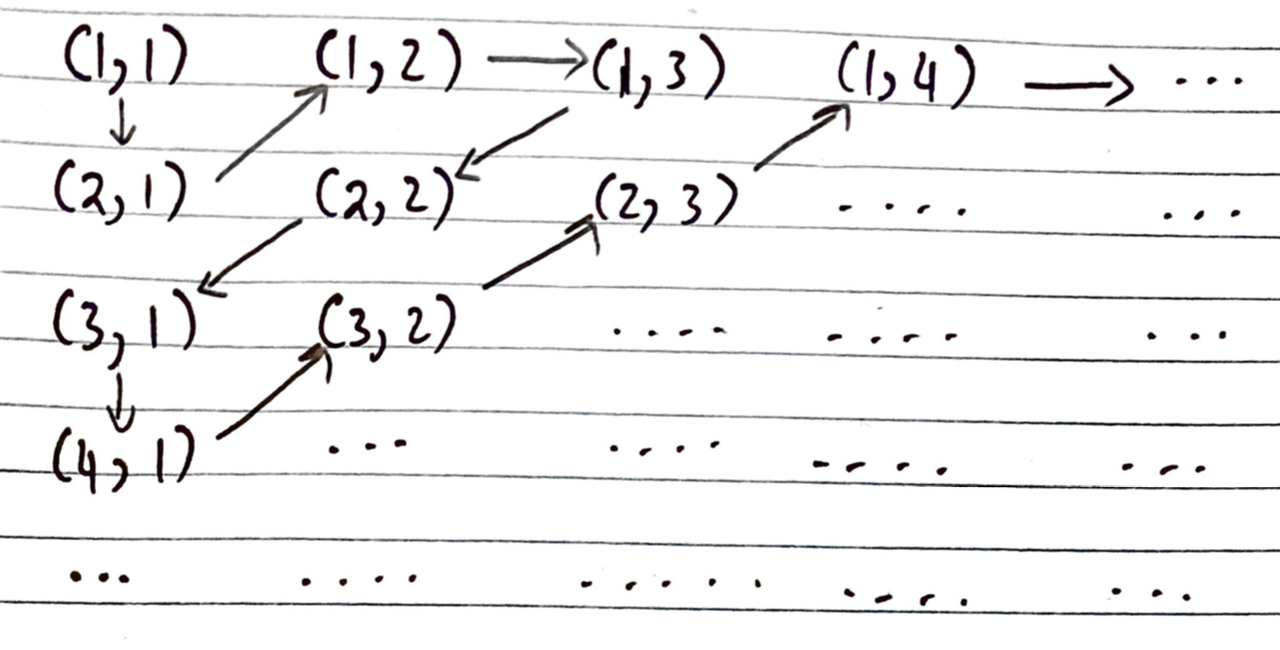
\includegraphics[scale = 0.6]{lastq.png}
        \end{center}

        This picture I have drawn is essentially $\mathbb{N}^2$ layed out in a grid format. We then traverse this grid in a zig-zag path. 

        We can then label each pair with how far down the path it is, so:

        $1 \to (1,1)$ \\
        $2 \to (2,1)$ \\ 
        $3 \to (1,2)$ \\ 
        $4 \to (1,3)$ \\ 
        $5 \to (2,1)$ \\ 
        $6 \to (3,1)$ \\ 
        $7 \to (4,1)$ \\
        $8 \to (3,2)$ \\ 
        $9 \to (2,3)$ \\ 
        $10 \to (1,4)$ \\
        and so forth...

        So since we can continue to draw more pairs of $\mathbb{N}^2$ in a grid format and zig zag through and map each natural number to a $(x,y)$ pair in this zig zag path, we essentially create a bijection.


        Another way of thinking about this picture is that we can imagine $\mathbb{N}$ to be a number line. If we traverse this path shown above in my picture we create another line. Both of these are lines are continuous and never end. 

        Since both of them are a line there must exist a bijection between them.




    \end{homeworkProblem}
    
    \pagebreak






    








    \end{document}